\documentclass[12pt]{jarticle}
\usepackage{a4wide}
\usepackage{amsmath}%数学記号
\usepackage{amssymb}%数学記号
\usepackage{epsfig}%図
\usepackage{latexsym}
\usepackage{supertabular}
\usepackage{graphicx}
\usepackage{color}
\usepackage{ascmac}
\usepackage{multicol}
\usepackage{ascmac}
\usepackage{systeme}
\usepackage{amsmath,cases}
\usepackage{float}
\usepackage{here}
\usepackage{mathrsfs}
\pagestyle{plain}

\newtheorem{theorem}{定理}[section]
\newtheorem{lemma}[theorem]{補題}
\newtheorem{proposition}[theorem]{命題}
\newtheorem{conjecture}[theorem]{予想}
\newtheorem{corollary}[theorem]{系}
\newtheorem{definition}[theorem]{定義}
\newtheorem{example}[theorem]{例}
\newtheorem{exercise}[theorem]{例題}
\newtheorem{problem}[theorem]{問}
\newtheorem{algorithm}[theorem]{アルゴリズム}
\newtheorem{remark}[theorem]{注意}

\def\qed{{\hfill$\square$}}
\def\proof{{\vspace{-0.3cm}f 証明: \,}}
\def\solution{{\vspace{-0.3cm}f 解: \,}}
\def\N{{\Bbb N}}
\def\Z{{\Bbb Z}}
\def\Q{{\Bbb Q}}
\def\R{{\Bbb R}}
\def\C{{\Bbb C}}
\def\F{{\Bbb F}}
\def\D{{\mathcal D}}
\def\mod{{\mathrm{mod\,\,}}}
\def\GL{{\mathrm{GL}}}
\def\GF{{\mathrm{GF}}}
\def\H{{\mathcal{H}}}

\setlength{\textwidth}{170mm}
\setlength{\textheight}{240mm}
\setlength{\oddsidemargin}{-5mm}
\setlength{\evensidemargin}{-5mm}
\setlength{\topmargin}{-10mm}
\setlength{\headheight}{0mm}
\setlength{\headsep}{10mm}

\title{確率統計特論}
\begin{document}
\maketitle
\section{ルベーグの優収束定理}
\begin{shadebox}
  定義: \ \ 可測集合$A$上の可測関数列${f_n}$は、$A$上各点収束するとする。\\ ある$A$上可測積分関数$g$が存在して、$\forall n$に対して、
  \begin{align*}
    |f_n(x)| \leq g(x) a.e x \in A
  \end{align*}
を満たすとき、
\begin{align*}
  \lim_{n \rightarrow \infty} \int_A f_n (x) dx = \int_A \lim_{n \rightarrow \infty}  f_n (x) dx
\end{align*}
\end{shadebox}

ポイントは$3$つ
\begin{itemize}
  \item ${f_n}$が各点収束すること
  \item $g$が${f_n}$の優関数であること
  \item $g$が可積分であること
\end{itemize}
これを期待値について考えると
\begin{shadebox}
  ($\Omega$,$\mathscr{F}$,$P$):確率空間\\ $X_n$,$n=1,2,\cdots$:確率変数\\
  に対して、
  \begin{itemize}
    \item $|X_n| \leq U,j = 1,2,\cdots $となる$U$が確率$1$で存在する。
    \item $\displaystyle \lim_{j \rightarrow \infty} X_n = X$が成立する。
  \end{itemize}
  このとき、$\displaystyle \lim_{n \rightarrow \infty} E[X_n] = E[\lim_{n \rightleftarrows \infty}X_n]$となる
\end{shadebox}

\section{期待値と極限が交換できない場合}
\begin{shadebox}
\begin{flalign*}
  \displaystyle
  &\Omega = (0,1),P:一様分布& \\ &X_n(\omega) = n(\omega \in (0,\frac{1}{n}))& \\ &X_n(\omega) = 0 (otherwise)&
\end{flalign*}
このとき$\displaystyle \forall n$に対して、$\displaystyle E[X_n] = 1$だが$\displaystyle \omega$に対して$\displaystyle X_{n}(\omega) \rightarrow 0$なので、\\ $\displaystyle \lim E[X_n] = 1,E[\lim X_n] = 0$
\end{shadebox}
\begin{figure}[H]
  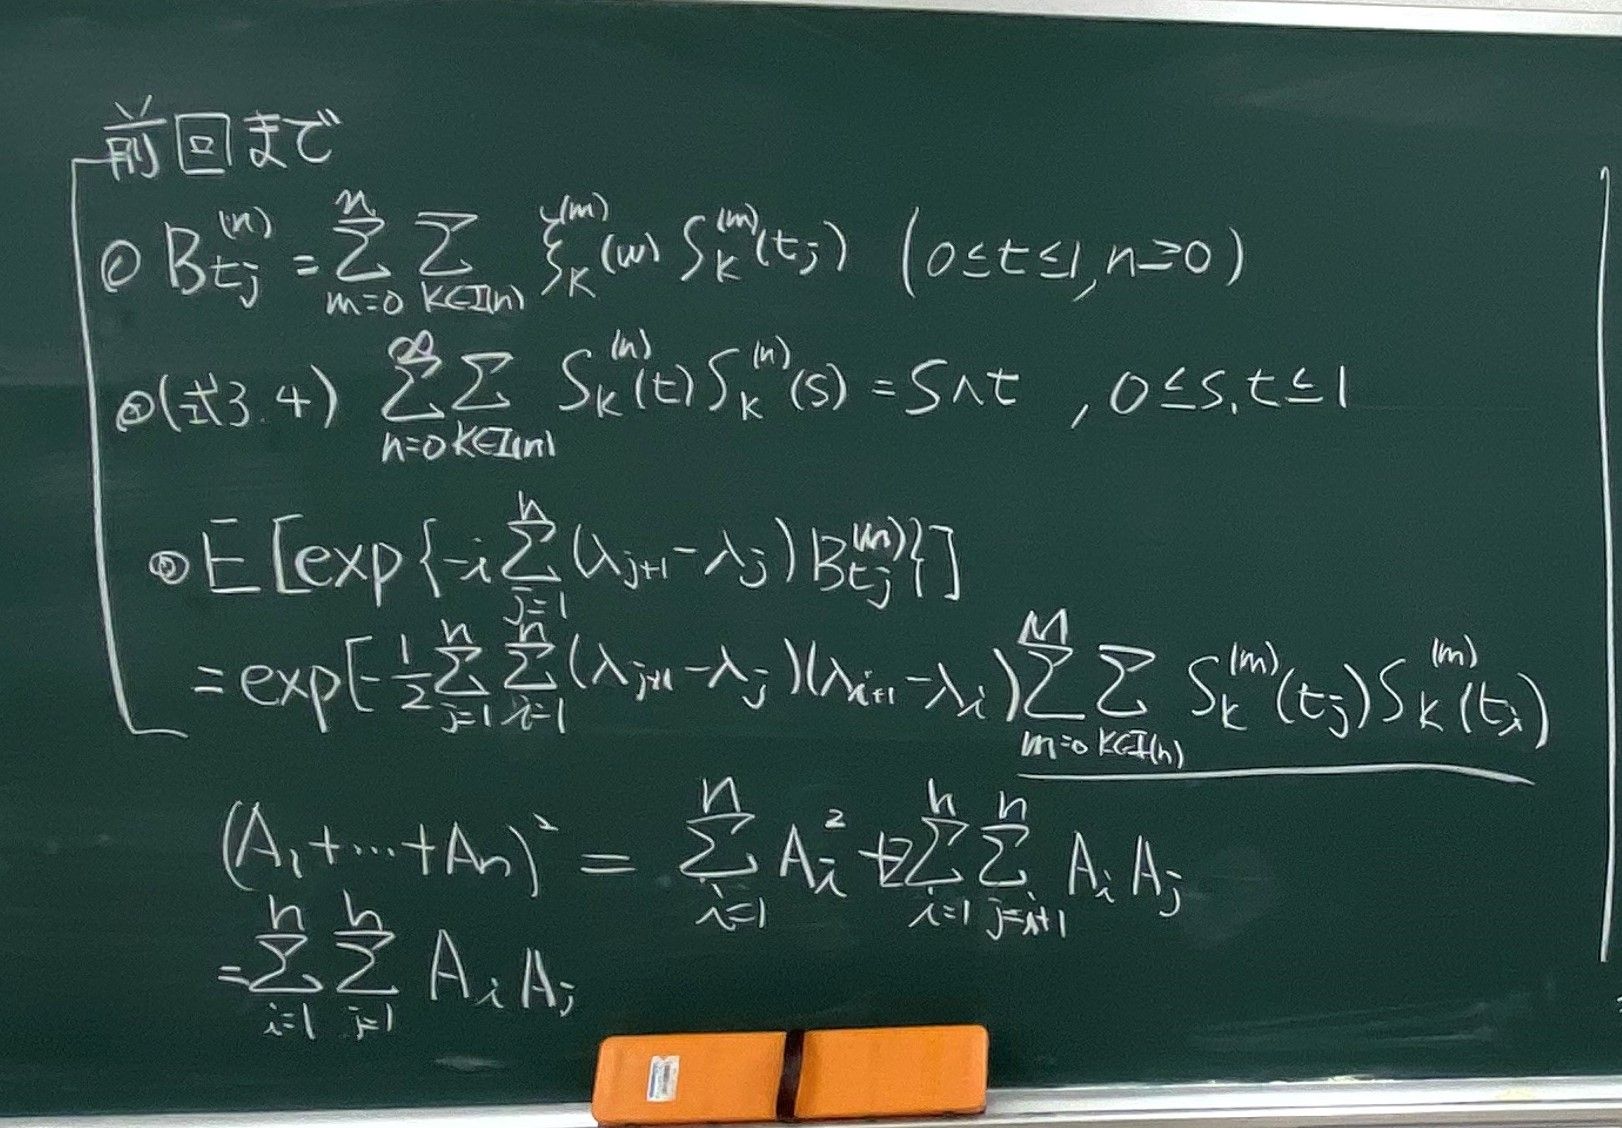
\includegraphics[bb = -7 1100 1 1,scale = 0.3]{黒板_1.png}
  \vspace{11.5cm}
  \caption{前回までに分かったこと}
\end{figure}


\end{document}
